\documentclass{article}

\usepackage{tikz}
\usetikzlibrary{positioning}
\usepackage{bera}% optional: just to have a nice mono-spaced font
\usepackage{listings}
\usepackage{xcolor}

\usepackage{uml}



\colorlet{punct}{red!60!black}
\definecolor{background}{HTML}{EEEEEE}
\definecolor{delim}{RGB}{20,105,176}
\colorlet{numb}{magenta!60!black}

\lstdefinelanguage{json}{
    basicstyle=\normalfont\ttfamily,
    numberstyle=\scriptsize,
    stepnumber=1,
    numbersep=8pt,
    showstringspaces=false,
    breaklines=true,
    literate=
     *{0}{{{\color{numb}0}}}{1}
      {1}{{{\color{numb}1}}}{1}
      {2}{{{\color{numb}2}}}{1}
      {3}{{{\color{numb}3}}}{1}
      {4}{{{\color{numb}4}}}{1}
      {5}{{{\color{numb}5}}}{1}
      {6}{{{\color{numb}6}}}{1}
      {7}{{{\color{numb}7}}}{1}
      {8}{{{\color{numb}8}}}{1}
      {9}{{{\color{numb}9}}}{1}
      {:}{{{\color{punct}{:}}}}{1}
      {,}{{{\color{punct}{,}}}}{1}
      {\{}{{{\color{delim}{\{}}}}{1}
      {\}}{{{\color{delim}{\}}}}}{1}
      {[}{{{\color{delim}{[}}}}{1}
      {]}{{{\color{delim}{]}}}}{1},
}

\title{Documentation ADM Project}
\author{Riccardo Bianchini, Andrea Canepa}
\date{\today}

\begin{document}

\maketitle
\tableofcontents
\newpage


\section{Introduction}
We would like to offer pubs' clients an application that helps them to choose
the best beer for their evenings. As we know, there are lots of types of
beers, each one different from the other because of a lot of factors,
weel-known by the connoisseurs. In detail we want to permit a smart set of
queries to make an aware choice based on technical parameters, in addition to
data analysis.

\newpage

\section{Conceptual schema}
This is an empty example of a conceptual schema, in real documentation i hope the result will be better

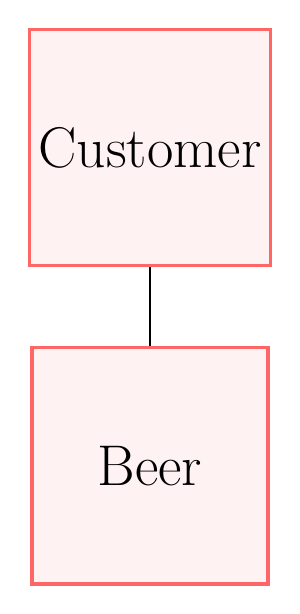
\begin{tikzpicture}[squarednode/.style={rectangle, draw=red!60, fill=red!5, very thick, minimum size=30mm},]

%Nodes

\node[squarednode] (Customer) {\huge{Customer}};
\node[squarednode] (Beer) [below=of Customer] {\huge{Beer}};
\draw[-] (Customer.south) -- (Beer.north);
\end{tikzpicture}

\newpage

\section{Workload}
\begin{itemize}
\item 
\item secondo

\end{itemize}



\newpage

\section{Logical schema}
This is a json- style example
\begin{lstlisting}[language=json,firstnumber=1]
{"menu": {
  "id": "file",
  "value": "File",
  "popup": {
    "menuitems": "List int"
  }
}}

\end{lstlisting}

\newpage


\umlClass[box=,reference=AmericanMan,stereotype=Uomo,import=,importedFrom=America,comment=A man from America]{American Man}{%
\umlAttribute[visibility=\#, type=State]{State}\umlAttribute[visibility=\#,default=Mc Donalds]{Favourite burger}}{%
\umlMethod[visibility=]{Watch TV}{}\umlMethod[visibility=-, returntype=int]{Vote}{Party party}}

\end{document}
